


% the process of capturing energy from the surrounding environment


% Energy harvesting has been demonstrated as a viable alternative for powering low-energy electronics systems, such as Internet of Things (IoT) devices and wireless sensor systems
% \cite{xuSelfpoweredRPMSensor2023}.


% In many cases, the output of energy harvesters is an alternating current (AC) requiring rectification in order to supply the electronic load. The rectifier design and selection can have a considerable influence on the energy harvesting system performance in terms of extracted output power and conversion losses


% The rapid advancement of the Internet of Things (IoT) and wireless sensor networks has revolutionized the monitoring of industrial, structural, and transportation systems. As the deployment of smart sensors continues to scale, ensuring a continuous and reliable power supply has become a critical bottleneck. Traditional battery-powered solutions present significant limitations, including finite lifespans, frequent maintenance requirements, logistics costs, and environmental concerns. In this context, energy harvesting—the process of capturing and converting ambient energy into usable electrical power—has emerged as a highly promising strategy to develop self-sustaining, autonomous sensor systems.

% Among the various ambient energy sources available, kinetic energy derived from rotational motion is particularly abundant in industrial machinery, vehicles, and urban infrastructure. Harvesting this rotational energy offers a consistent power source for monitoring critical moving components, such as bearings, wheels, and drive shafts. Electromagnetic and variable reluctance energy harvesters have proven to be robust and effective technologies for this purpose, capable of operating efficiently across different speed ranges without requiring complex mechanical attachments.

% However, the practical implementation of rotational energy harvesting systems introduces several engineering challenges. At low rotational speeds, the generated power is often limited and highly variable, requiring highly efficient power management and rectification circuits to supply direct current (DC) to electronic loads. Additionally, the mechanical integration of these harvesters must be carefully designed to minimize any adverse effects on the host system, such as unwanted vibrations, acoustic noise, or torque ripple. Overcoming these barriers requires a comprehensive approach that combines mechanical design, electromagnetic optimization, and advanced electronic circuitry.

% This thesis aims to explore the principles, design, and optimization of energy harvesting systems for rotational applications. By analyzing the fundamental trade-offs between mechanical constraints, energy conversion efficiency, and power output, this work seeks to evaluate and propose improved architectures. Ultimately, the objective is to advance the development of highly efficient, reliable, and self-powered sensor networks capable of seamlessly integrating into modern smart environments.


% . Motivazione globale
% Perché l'energy harvesting è rilevante oggi — crescita dei dispositivi IoT, edge computing, sensori wireless, wearable. Il problema dell'alimentazione a batteria (manutenzione, sostituzione, sostenibilità). La domanda: esiste un'alternativa?
% 2. Cos'è l'energy harvesting
% Definizione, principio generale. Energia "ambientale" come fonte: vibrazione, termica, RF, solare, piezoelettrica. Vantaggi chiave: autonomia, manutenzione zero, scalabilità.
% 3. Contesto storico
% Quando nasce e perché — puoi partire dai primi generatori termoelettrici degli anni '50/'60 (es. nelle sonde spaziali), poi il boom con la miniaturizzazione elettronica e l'IoT degli anni 2000.
% 4. Principali tecnologie esistenti
% Una panoramica delle famiglie principali: piezoelettrico, elettromagnetico, elettrostatico, termoelettrico, fotovoltaico, RF harvesting. Non serve entrare nel dettaglio — quello va nei capitoli successivi.
% 5. Sfide aperte (questo ti consiglio di aggiungere)
% Densità di potenza ancora bassa, dipendenza dalle condizioni ambientali, circuiti di power management, integrazione con i carichi. Questo giustifica la ricerca attiva nel campo — e prepara il terreno per il tuo contributo.
% 6. Obiettivo e struttura della tesi (fondamentale)
% Di cosa si occupa esattamente la tua tesi, qual è il contributo originale, e come sono organizzati i capitoli. Questo è l'ultimo paragrafo dell'introduzione e il lettore lo aspetta.

\chapter{Introduction}

\section{Motivation}

The number of wireless sensor networks (WSNs) and Internet 
of Things (IoT) devices has grown rapidly in recent years, 
raising a fundamental question: how to power all these 
devices without replacing batteries or requiring constant 
maintenance. Recent advances in low-power electronics have 
reduced the energy consumption of sensor nodes to the range 
of tens to hundreds of microwatts 
\cite{roundyStudyLowLevel2003a}. At such low power levels, 
it becomes possible to power these devices by extracting 
energy from the surrounding environment, removing the need 
for batteries and allowing the network to operate 
indefinitely.

Batteries are the most common power source for WSN nodes, 
but they have well-known limitations. In many applications, such as structural health monitoring, industrial 
machinery surveillance, or medical implants, replacing or 
recharging depleted batteries is difficult or simply not 
possible \cite{grossiEnergyHarvestingStrategies2021}. Using 
larger batteries to extend the device lifetime increases the 
size of the system, which is often not acceptable. In 
addition, the environmental cost of battery and the consequent 
maintenance of large-scale networks are serious 
obstacles to the widespread use of WSNs 
\cite{leonavilaEnergyHarvestingTechniques2025}.

Energy harvesting offers a practical solution to these 
problems. Instead of storing a fixed amount of energy, 
harvesting systems collect energy from sources available in 
the environment such as sunlight, heat gradients, mechanical 
vibrations, or radio frequency signals and convert it 
into electrical power to supply an electronic system.

Among all available energy sources, mechanical vibrations 
have received the most attention in the research community, 
accounting for more than half of publications in this field 
\cite{leonavilaEnergyHarvestingTechniques2025}. 
Piezoelectric, triboelectric, and electromagnetic transducers 
are the most widely used mechanisms, each with different 
trade-offs in output voltage, power density, and complexity 
\cite{roundyStudyLowLevel2003a, 
grossiEnergyHarvestingStrategies2021}.
Figure \ref{fig:transducer_distribution} shows the 
distribution of recent publications about transducer types, 
highlighting the dominance of mechanical energy harvesting 
approaches.



\begin{figure}[htbp]
\centering
\definecolor{colHeat}{RGB}{55,138,221}
\definecolor{colLight}{RGB}{239,159,39}
\definecolor{colEMF}{RGB}{151,196,89}
\definecolor{colRF}{RGB}{212,83,126}
\definecolor{colMech}{RGB}{127,119,221}
\definecolor{colChem}{RGB}{136,135,128}
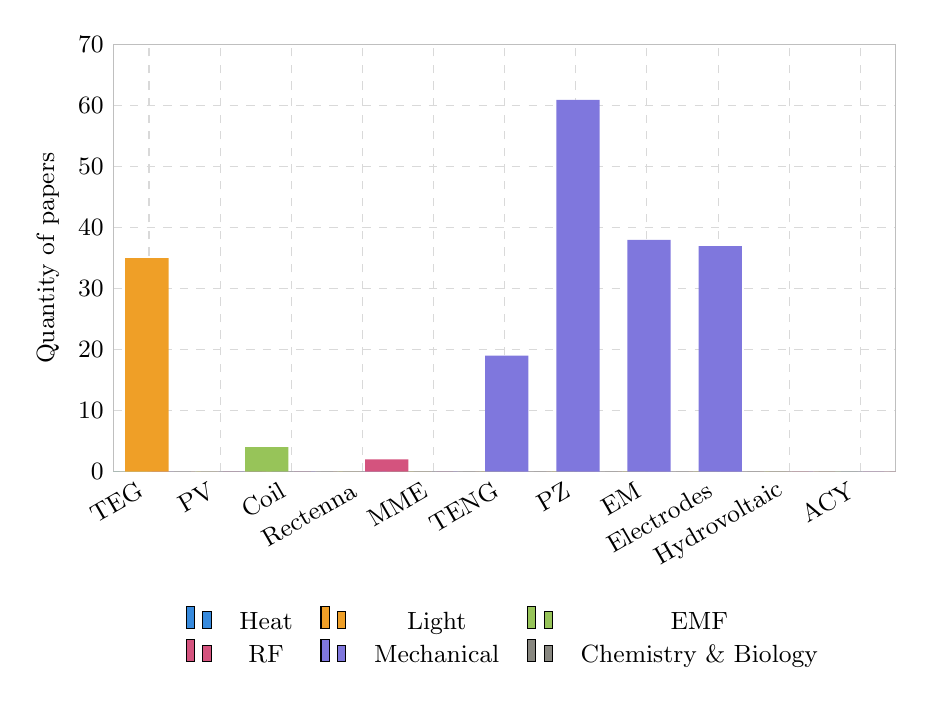
\begin{tikzpicture}
\begin{axis}[
    ybar,
    bar width        = 0.55cm,
    width            = 0.95\textwidth,
    height           = 7cm,
    enlarge x limits = 0.05,
    ylabel           = {Quantity of papers},
    ylabel style     = {font=\small},
    symbolic x coords = {TEG, PV, Coil, Rectenna, MME,
                          TENG, PZ, EM, Electrodes, Hydrovoltaic, ACY},
    xtick            = data,
    xticklabel style = {font=\small, rotate=30, anchor=east},
    ymin = 0, ymax   = 70,
    ytick            = {0,10,20,30,40,50,60,70},
    yticklabel style = {font=\small},
    grid             = major,
    grid style       = {dashed, gray!30},
    axis line style  = {gray!50},
    tick style       = {draw=none},
    legend style     = {
        at={(0.5,-0.30)},
        anchor=north,
        legend columns=3,
        font=\small,
        draw=none,
        column sep=0.8em
    },
]

\addplot[fill=colHeat, draw=none] coordinates {
    (TEG,24)(PV,0)(Coil,0)(Rectenna,0)(MME,0)
    (TENG,0)(PZ,0)(EM,0)(Electrodes,0)(Hydrovoltaic,0)(ACY,0)};
\addlegendentry{Heat}

\addplot[fill=colLight, draw=none] coordinates {
    (TEG,0)(PV,35)(Coil,0)(Rectenna,0)(MME,0)
    (TENG,0)(PZ,0)(EM,0)(Electrodes,0)(Hydrovoltaic,0)(ACY,0)};
\addlegendentry{Light}

\addplot[fill=colEMF, draw=none] coordinates {
    (TEG,0)(PV,0)(Coil,4)(Rectenna,0)(MME,0)
    (TENG,0)(PZ,0)(EM,0)(Electrodes,0)(Hydrovoltaic,0)(ACY,0)};
\addlegendentry{EMF}

\addplot[fill=colRF, draw=none] coordinates {
    (TEG,0)(PV,0)(Coil,0)(Rectenna,2)(MME,0)
    (TENG,0)(PZ,0)(EM,0)(Electrodes,0)(Hydrovoltaic,0)(ACY,0)};
\addlegendentry{RF}

\addplot[fill=colMech, draw=none] coordinates {
    (TEG,0)(PV,0)(Coil,0)(Rectenna,0)(MME,19)
    (TENG,61)(PZ,38)(EM,37)(Electrodes,0)(Hydrovoltaic,0)(ACY,0)};
\addlegendentry{Mechanical}

\addplot[fill=colChem, draw=none] coordinates {
    (TEG,0)(PV,0)(Coil,0)(Rectenna,0)(MME,0)
    (TENG,0)(PZ,0)(EM,0)(Electrodes,0)(Hydrovoltaic,0)(ACY,0)};
\addlegendentry{Chemistry \& Biology}

\end{axis}
\end{tikzpicture}
\caption{Distribution of papers based on transducer type.
Adapted from \cite{leonavilaEnergyHarvestingTechniques2025}.}
\label{fig:transducer_distribution}
\end{figure}



Energy harvesting systems are generally divided into two 
categories \cite{grossiEnergyHarvestingStrategies2021}: 
systems that use the harvested energy immediately 
(\emph{Harvest-Use}), and systems that store it first in a 
battery or supercapacitor before supplying it to the node 
(\emph{Harvest-Store-Use}). The second approach is far more 
common, since most energy sources are not continuously 
available and some form of storage is needed to guarantee 
uninterrupted operation.


\section{Energy Harvesting Systems}

An energy harvesting system is made of three components
that work in sequence, as illustrated in
Figure \ref{fig:BD_EHS}.

\begin{itemize}
    \item \emph{Transducer}: converts the ambient energy into an electrical signal.
    \item \emph{Power conditioning circuit}: perform AC-DC conversion, impedance matching and voltage regulation. A typical implementation combines a rectifier circuit with a power management integrated circuit (PMIC) \cite{xuSystemImplementationTradeOffs2021}.
    \item \emph{energy storage element}: is used to keep the device operating for a certain amount of time even if the source is week or no more present. Such element can be a capacitor/super capacitor or a rechargeable battery \cite{roundyStudyLowLevel2003a}.
\end{itemize}



%Inserire uno schema a blocchi di transducer, pcc e nenrgy storage
\begin{figure}[htbp]
\centering
\caption{Block diagram of a typical energy harvesting system.}
\label{fig:BD_EHS}
\end{figure}



The performance of the entire system depends in particular on
the transducer. Its design must be matched to the
characteristics of the ambient source as well as to the power need
of the target device. A transducer that is well suited to
one environment may perform poorly in another, which is why
the choice of transduction mechanism is the central design
decision in any harvesting application \cite{grossiEnergyHarvestingStrategies2021}.

Designing a good harvesting system is not just about 
getting the most power out of it. The system must work 
reliably in real conditions, where the energy source can 
be irregular or unpredictable. At the same time, it must 
be small, cheap, and easy to integrate into the target 
device \cite{grossiEnergyHarvestingStrategies2021}. Finding 
the right balance between these requirements is the main 
challenge in this field, and it has led to the development 
of many different solutions, as discussed in the following 
sections.

\section{Performance metrics}

A key challenge in evaluating energy harvesting systems is 
choosing the right performance metrics. Xu et 
al.\cite{xuSystemImplementationTradeOffs2021} propose two metrics 
for this purpose. The first is the \emph{power conversion 
efficiency} (PCE), which measures how much of the power 
entering the interface circuit actually reaches the output:


\begin{equation}
    \text{PCE} = \eta_\text{Rec} \cdot \eta_\text{DC-DC} 
    = \frac{P_\text{out}}{P_\text{in}}.
    \label{eq:pce}
\end{equation}


The second is the \emph{power extraction efficiency} (PEE), 
which compares the output power to the maximum power the 
transducer could deliver under ideal conditions:


\begin{equation}
    \text{PEE} = \frac{P_\text{out}}{P_\text{max}} 
    = \frac{P_\text{in}}{P_\text{max}} \cdot \text{PCE}.
    \label{eq:pee}
\end{equation}


The difference between the two is important. A circuit can 
convert power efficiently (high PCE) while still wasting 
much of what the transducer could produce, if the circuit 
itself is not able to work in the optimal operating 
point. For this reason, PEE is a more useful metric when the 
goal is to maximise the total power delivered to the 
load \cite{xuSystemImplementationTradeOffs2021}.



\section{Main Transduction Technologies}

Mechanical vibrations can be converted into electrical 
energy through four main transduction mechanisms: 
piezoelectric, electromagnetic, electrostatic, and 
triboelectric. Each of them works in a different way and 
comes with its own advantages and 
limitations \cite{mitchesonEnergyHarvestingHuman2008, beebyEnergyHarvestingVibration2006}.

\subsection*{Piezoelectric}
Piezoelectric transducers produce a voltage when a 
material is mechanically deformed. The most common design
is a cantilever beam with a piezoelectric layer on top:
when the beam vibrates, the material deforms and
generates an electric charge. This approach gives a
high output voltage and does not need a magnet or
moving parts, which makes it easy to integrate into small 
devices \cite{antonReviewPowerHarvesting2007}. The main drawback is that
piezoelectric materials are fragile and may crack under
large deformations. Also, the output drops quickly
when the vibration frequency moves away from the 
resonant frequency of the 
beam \cite{roundyStudyLowLevel2003a}.


\subsection*{Electromagnetic}
Electromagnetic transducers generate a voltage by
moving a coil near a permanent magnet. This is the
same principle used in large electrical generators,
applied at a small scale. These harvesters tend to
produce a low voltage but can deliver a relatively
high current, which makes them a good choice when
power output is the main goal.
One limitation is that the coil and magnet must move
relative to each other, which can be hard to achieve
in applications involving large or slowly rotating
objects \cite{mitchesonEnergyHarvestingHuman2008}.

\subsection*{Electrostatic}
Electrostatic transducers work by changing the
capacitance between two conductive plates as they
move. When the plates get closer or further apart
due to vibration, the stored electrical energy
changes and can be extracted as useful power.
This approach is easy to manufacture using standard
microfabrication processes, making it attractive for
very small devices. However, it requires an external
voltage or a pre-charged material to get started,
which adds complexity to the
system \cite{mitchesonEnergyHarvestingHuman2008, beebyEnergyHarvestingVibration2006}.

\subsection*{Triboelectric}
Triboelectric transducers use contact between two
different materials to generate surface charges.
When the materials touch and then separate, charges
build up and can drive a current through an external
circuit. This type of harvester, known as a
triboelectric nanogenerator (TENG), was first
demonstrated by Fan et al.\cite{fanFlexibleTriboelectricGenerator2012} and
has attracted a lot of interest because it can be
made from cheap, flexible materials and works well
at low frequencies, such as those produced by human
motion. The main weaknesses are sensitivity to
humidity and wear of the contact surfaces over
time \cite{leonavilaEnergyHarvestingTechniques2025}.

Among these four mechanisms, no single technology is 
universally superior. The best choice depends on the 
specific application, the characteristics of the available 
vibration source, and the constraints on size and cost. 
This comparison motivates the investigation of 
alternative approaches, including variable reluctance 
transduction, which is discussed in the following section.




\section{The Variable Reluctance Principle}


Variable reluctance energy harvesting (VREH) is a type of
electromagnetic energy harvesting based on Faraday's law
of induction. The transducer consists of three main parts:
a permanent magnet, a pickup coil wound around a
ferromagnetic pole piece, and a toothed ferromagnetic
wheel that rotates nearby. When a tooth on the wheel
aligns with the pole piece, the magnetic flux through the
coil reaches its maximum value. When the gap between two
teeth faces the pole piece, the flux drops to its minimum.
This periodic variation in flux induces an alternating
voltage across the coil, with a frequency that depends on
the rotational speed and the number of teeth on the
wheel \cite{xuSurveyVariableReluctance2018}:
%
\begin{equation}
    f_c = \omega \, N_t,
    \label{eq:vreh_freq}
\end{equation}
%
where $\omega$ is the rotational speed in rad/s and $N_t$
is the number of teeth on the weel. Following Faraday's law, the output
power of the transducer delivered to a matched load can be expressed
as \cite{xuDesignModelingOptimization2019a}:
%
\begin{equation}
    P_L = \frac{N_\text{Coil}^2}{8R_\text{Coil}}
    \Delta_\phi^2
    \left[\frac{\omega N_\text{Tooth}}{2\pi}\right]^2,
    \label{eq:vreh_power}
\end{equation}
%
where $N_\text{Coil}$ is the number of coil turns,
$R_\text{Coil}$ is the coil resistance, $\Delta_\phi$ is
the magnetic flux difference between the aligned and
unaligned positions, and $N_\text{Tooth}$ is the number of
teeth. This expression shows that the output power grows
with the square of the rotational speed, and that it can
be increased by maximising the flux difference and the
number of coil turns, or by reducing the coil resistance.

What makes VREH different from most other electromagnetic
harvesters is that neither the magnet nor the coil needs
to move. The flux variation is caused entirely by the
relative motion between the toothed wheel and the pickup units.
This removes the need for a mechanical connection between the 
rotating part and the harvester, which is an advantage. It also
means that the device is easy to scale: changing the shaft
diameter mainly affects the size of the toothed wheel,
while the pickup unit can stay the
same \cite{xuDesignModelingOptimization2019a}. In contrast, traditional
electromagnetic generators require scaling of the magnets
or coils, which becomes costly for large shafts or slow
rotational speeds.

At low rotational speeds, the output voltage and frequency
are both small, which makes the design of the interface
circuit more critical \cite{xuSystemImplementationTradeOffs2021}.
At the same time, low-speed applications are exactly where
VREH has the clearest advantage over other electromagnetic
harvesters, since these typically require a relative
displacement between coil and magnet that is hard to
achieve at low speeds \cite{mitchesonEnergyHarvestingHuman2008}.

Its application to energy harvesting is more recent. Kroener et
al. \cite{kroenerVariableReluctanceHarvester2013} were among the first to study a
VREH specifically designed for energy harvesting in railway
monitoring, showing that the principle could reliably power
wireless sensor nodes from the motion of passing train
wheels. Since then, the approach has been explored in a
growing number of industrial and structural monitoring
applications \cite{xuSurveyVariableReluctance2018, xuDesignModelingOptimization2019a}.





\section{State of the Art of VREH}


The first applications of the variable reluctance principle
to energy harvesting appeared in the context of railway
monitoring. Kroener et al. \cite{kroenerVariableReluctanceHarvester2013} demonstrated
that a VREH placed beside a rail track could generate
enough power from the passage of train wheels to supply a
wireless sensor node, reporting a peak output power of
around $5.9$ mW at a simulated train speed of $81.5$ Km/h.
This work showed for the first time that the variable
reluctance principle could be practically used as an energy source
rather than just a measurement transducer.

A systematic comparison of VREH topologies was later
carried out by Xu et al. \cite{xuSurveyVariableReluctance2018}, who surveyed
the structures proposed in the literature and evaluated
them in terms of output power and power density for
low-speed rotating applications. The study identified the
\emph{m-shaped} pickup unit, which uses two opposing
permanent magnets and a centre pole piece, as the
topology with the highest volumetric power density among
all structures considered. This result motivated a
detailed design study of the m-shaped VREH, in which
the influence of three key geometric parameters was
investigated: the coil height $h_\text{Coil}$, the tooth
height $h_\text{Tooth}$, and the magnet height
$h_\text{M}$ \cite{xuDesignModelingOptimization2019a}. The study
showed that these parameters involve trade-offs under size
constraints, and provided a numerical optimisation method
based on finite element analysis (FEA). The optimised
structure reached output powers between 0.12 mW and
22 mW at rotational speeds of 5\,rpm to 60 rpm within
a volume constraint of 43.5 cm $^3$, which is sufficient
to power a range of duty-cycled wireless sensor
systems \cite{xuDesignModelingOptimization2019a}.

A practical challenge in VREH systems is that the
transducer produces a low-voltage alternating output,
which must be rectified and conditioned before it can
supply any systems. At low rotational speeds, the output
voltage can be well below 1 V, which makes the choice of
rectifier circuit critical. Xu et
al. \cite{xuSystemImplementationTradeOffs2021} compared three
passive rectifier topologie: a full-wave bridge
rectifier (FWR), a voltage doubler (VD), and a negative
voltage converter (NVC), all on the same VREH system at
speeds between 5 rpm and 20 rpm. The results showed
that the VD achieved the best power extraction efficiency
at low speeds, reaching a PEE of 40-60\%, while the NVC
outperformed it above 18 rpm. The FWR showed the lowest
performance across all conditions, with PEE values of only
20-40\%. These results confirm that the interface circuit
is not just a passive element but actively affects how
much power the transducer can deliver to the load.

These studies show that VREH is a mature
and well-understood technology for low-speed rotational
applications, with demonstrated power levels sufficient
for a variety of wireless sensing applications. The most recent
step forward in this direction is the multi-phase VREH
proposed by Wu et al. \cite{wuMultiPhaseVariableReluctance2024}, which
integrates six m-shaped pickup units into a bearing hub
unit for large commercial vehicles, reaching output powers
between 0.46 W and 4.77 W at rotational speeds of
100 to 400 RPM. This significant increase in output power
opens new possibilities for powering more demanding
condition monitoring systems. However, it also introduces
new challenges in the design of the power conditioning
circuit, which must handle six independent AC outputs
with different phases and varying voltage levels depending
on the rotational speed. These challenges are discussed in
the next section.


\section{Open Challenges}


Despite the progress described in the previous sections,
several challenges remain open in the design of VREH
systems. This section focuses on those that are most
relevant to the work presented in this thesis.

\subsection*{Power conditioning for multi-phase outputs}
Single-phase VREH systems produce one alternating
voltage signal that must be rectified and converted into a
stable DC supply. This problem has been studied in detail
for low-speed single-phase harvesters, where the choice
of rectifier topology has a significant impact on the
power extraction efficiency \cite{xuSystemImplementationTradeOffs2021}.


Many studies have investigated the design of power 
conditioning circuits for single-phase
energy harvesters. The most common approach combines 
a rectification stage with a DC-DC converter, such as a 
Buck or Boost circuit, to regulate the output voltage to 
a level suitable for the target load \cite{yuSingleStageAC2016,yuDiscontinuousConductionMode2017a,hsiehSimpleBidirectionalBridgeless2014,dayalNewSingleStage2010}. However, these 
solutions are designed for a single AC input and cannot 
be directly applied to a multi-phase harvester such as 
the MP-VREH, where six independent AC signals must 
be processed simultaneously.

Furthermore, many of these solutions do not include a
startup circuit or a control system, which are both
essential for the reliable operation of the power
conditioning circuit in practice. Without a startup
circuit, the system is not able to start operating when
the harvested voltage is initially too low to power the
control electronics. Without a control system, the
circuit cannot adapt to changes in the rotational speed
or load conditions, which are essential in real-world
applications.

This gap in the literature 
motivates the investigation presented in this thesis.

When the number of pickup units increases,
as in the multi-phase VREH proposed by Wu et
al. \cite{wuMultiPhaseVariableReluctance2024}, which uses six m-shaped
pickup units arranged around a common toothed wheel,
the power conditioning problem becomes considerably
more complex. Each pickup unit produces an independent
AC output with a different phase and the six signals are evenly
spaced in time by $60^\circ$ phase shift.
This means that standard single-phase rectifier
solutions cannot be directly applied, and that the
interface circuit must be designed to handle multiple AC inputs efficiently.

\subsection*{Low output voltage at low speed}
A fundamental limitation of VREH transducers is that
the output voltage scales with rotational speed. At low
speeds, the induced voltage may be well below 1 V, which
makes rectification difficult because conventional diode
bridges lose a significant fraction of the available voltage
across their forward drops \cite{xuSystemImplementationTradeOffs2021}.
In a multi-phase system, this problem affects all six
phases simultaneously. Finding a rectifier topology that
works efficiently across a wide speed range, from the
minimum speed at which the harvester can sustain the
load, up to the maximum operating speed, is therefore
a key design requirement.

\subsection*{Impedance matching under variable conditions}
The maximum power that a VREH can deliver to a load
is achieved when the load impedance is matched to the
internal impedance of the pickup coil. This matching
condition depends on the rotational speed, because the
electrical frequency of the output signal changes with
speed. For a single-phase harvester, Xu et
al. \cite{xuDesignModelingOptimization2019a} showed that a fixed
resistive load leads to an approximately linear increase
in output power with speed, whereas a complex conjugate
matched load, which compensates for the inductive
component of the coil, could further increase the
output power, especially at higher speeds. In a six-phase
system, achieving dynamic impedance matching for all
phases simultaneously adds a further layer of complexity
to the interface circuit design.

\section{Harvester Specifications and Research Objective}
\label{sec:mpvreh_specs}

The work presented in this thesis is based directly on
the MP-VREH proposed by Wu et al. \cite{wuMultiPhaseVariableReluctance2024}.
The electrical characteristics of a single pickup unit,
obtained from the transducer model, are summarised in
Table \ref{tab:vreh_par}. These values are used
throughout this work as the reference operating
conditions for the design and evaluation of the proposed
power conditioning circuits.

\begin{table}[htbp]
    \centering

    \begin{tabular}{cccccc}
        \toprule
        RPM & $f$ (Hz) & $V_\text{Lpk}$ (V) & $R_\text{coil}$ ($\Omega$) &$L_\text{coil}$ (mH) & $P_o$ (W) \\
        \midrule
        100 & 36.7  & 0.91 & 6 & 21.68 & 0.41 \\
        200 & 73.3  & 1.35 & 6 & 21.46 & 0.91 \\
        300 & 110.0 & 1.59 & 6 & 21.27 & 1.26 \\
        400 & 146.7 & 1.74 & 6 & 21.12 & 1.51 \\
        \bottomrule
    \end{tabular}
    \caption{Electrical parameters of a single MP-VREH
             pickup unit at different rotational speeds.}
    \label{tab:vreh_par}
\end{table}

All values in Table \ref{tab:vreh_par} were obtained under
impedance-matched load conditions. $V_\text{Lpk}$ refers to
the peak voltage across the load, and $P_o$ is the average
power dissipated in the load.

The overall system consists of six pickup units arranged
in space so that they are electrically phase-shifted by
$60^\circ$ from one another.

These challenges motivate the work presented in this
thesis, which focuses on the design and evaluation of
power conditioning circuits for the six-phase MP-VREH
described above. The goal is to identify the interface
circuit topology that maximises the power delivered to
the load across the relevant operating speed range of
100 to 400 RPM (20-80 Km/h), corresponding to typical driving
conditions of large commercial vehicles, for exaple buses.